
\documentclass[conference]{IEEEtran}
\usepackage[T1]{fontenc}
\usepackage[utf8]{inputenc}
\usepackage[english]{babel}
\usepackage{graphicx}
\usepackage{amsmath}
\usepackage{booktabs}
\usepackage{cite}

\title{Kuantum Bilgisayarların Güçlü Şifreleme Sistemlerine Etkisi ve Post-Kuantum Geçiş Analizi}

\author{
\IEEEauthorblockN{Talay Vural, Muharrem Enes Sönmez, Ramazan Yusuf Ercan, Mahmut Burak Gök}
\IEEEauthorblockA{
Bilgisayar Programcılığı Bölümü\\
Türkiye\\
}
}

\begin{document}
\maketitle

\begin{abstract}
Kuantum bilgisayarların ölçeklenmesi, özellikle RSA ve Eliptik Eğri Kriptografisi (ECC) gibi açık anahtarlı şifreleme sistemlerini hedefleyen Shor algoritması nedeniyle mevcut siber güvenlik altyapısı için stratejik bir risk oluşturmaktadır.
Bu çalışmada MP1--MP5 mini projeleri tek bir raporda birleştirilmiş; problem ve hipotez (MP1), literatür taraması (MP2), açık veri seti ile veri toplama (MP3), performans analizi ve görselleştirme (MP4) ve sonuç/öneriler (MP5) IEEE biçiminde sunulmuştur.
Örnek bir KEM (Key Encapsulation Mechanism) benchmark veri seti üzerinden algoritmaların toplam süre--çıktı boyutu dengesi incelenmiş ve post-kuantum kriptografiye geçiş için uygulanabilir öneriler üretilmiştir.
\end{abstract}

\begin{IEEEkeywords}
Quantum Computing, Cybersecurity, Shor Algorithm, Post-Quantum Cryptography, NIST PQC, KEM Benchmarks
\end{IEEEkeywords}

\section{MP1: Problem ve Hipotez}
Günümüzde internet güvenliğinin büyük bir kısmı, açık anahtarlı kriptografi (RSA/ECC) ve simetrik şifreleme (AES gibi) bileşenlerine dayanmaktadır.
RSA/ECC, asal çarpanlara ayırma ve ayrık logaritma gibi klasik bilgisayarlar için hesaplama maliyeti yüksek problemlere dayanır.
Ancak Shor algoritması bu problemleri kuantum bilgisayarda polinom zamanda çözebilir \cite{shor1994}.
Bu nedenle, yeterince büyük ve hataya dayanıklı kuantum bilgisayarların geliştirilmesi durumunda, mevcut PKI altyapısının temel varsayımları zayıflayacaktır.

\textbf{Hipotez:} Kuantum ölçeklenmesi ile RSA/ECC pratik güvenliğini kaybederken, post-kuantum kriptografi (PQC) temelli KEM algoritmaları güvenli anahtar değişimi için uygulanabilir bir alternatif sunar; fakat güvenlik seviyesi arttıkça performans (süre) ve bant genişliği (ciphertext boyutu) arasında belirgin bir takas oluşur.

\section{MP2: Literatür Taraması}
Kuantum tehdit literatürü iki temel eksende özetlenebilir: (i) açık anahtarlı şemalara yönelik Shor tabanlı saldırılar \cite{shor1994}, (ii) simetrik şemalarda anahtar arama maliyetini yaklaşık karekök mertebesinde azaltan Grover araması \cite{grover1996}.
Bu çerçevede, simetrik algoritmalarda anahtar uzunluklarının artırılması önerilirken, açık anahtarlı sistemlerde doğrudan algoritma değişimi gerekmektedir.

Standartlaşma tarafında NIST, post-kuantum kriptografi standardizasyon sürecini yürütmekte ve KEM/İmza aileleri için aday algoritmaları değerlendirmektedir \cite{nistpqc}.
NISQ (Noisy Intermediate-Scale Quantum) dönemi tartışmaları, kısa vadede tehditin sınırlı olsa da ``harvest-now, decrypt-later'' riskinin stratejik önem taşıdığını vurgular \cite{preskill2018}.
Dolayısıyla kurumların kripto çevikliği (crypto agility) ve hibrit geçiş planları kritik hale gelmiştir.

\section{MP3: Veri Toplama}
Bu çalışmada MP3 aşaması kapsamında açık bir veri seti kullanılmıştır.
Veri seti, çeşitli post-kuantum KEM algoritmaları için \emph{keygen}, \emph{encap} ve \emph{decap} zamanları (ms) ile \emph{ciphertext\_length} gibi metrikleri içeren benchmark kayıtlarından oluşmaktadır \cite{kagglebench}.
Toplam kayıt sayısı 37,004 olup her kayıt; algoritma adı, güvenlik seviyesi, süre metrikleri ve çıktı boyutu gibi alanları içermektedir.
Veride eksik değer gözlenmemiş; doğruluk alanı (\emph{correctness}) tüm örneklerde \emph{True} raporlanmıştır.

\section{MP4: Analiz ve Görselleştirme}
Analiz sürecinde algoritmalar güvenlik seviyesi bazında gruplanmış ve ortalama toplam süre ile ortalama ciphertext boyutu karşılaştırılmıştır.
Şekil~\ref{fig:kem} toplam süre--ciphertext boyutu ilişkisini göstermekte; Tablo~\ref{tab:toplvl1} ise güvenlik seviyesi 1 için en hızlı algoritmaların özetini vermektedir.

\begin{figure}[htbp]
\centering
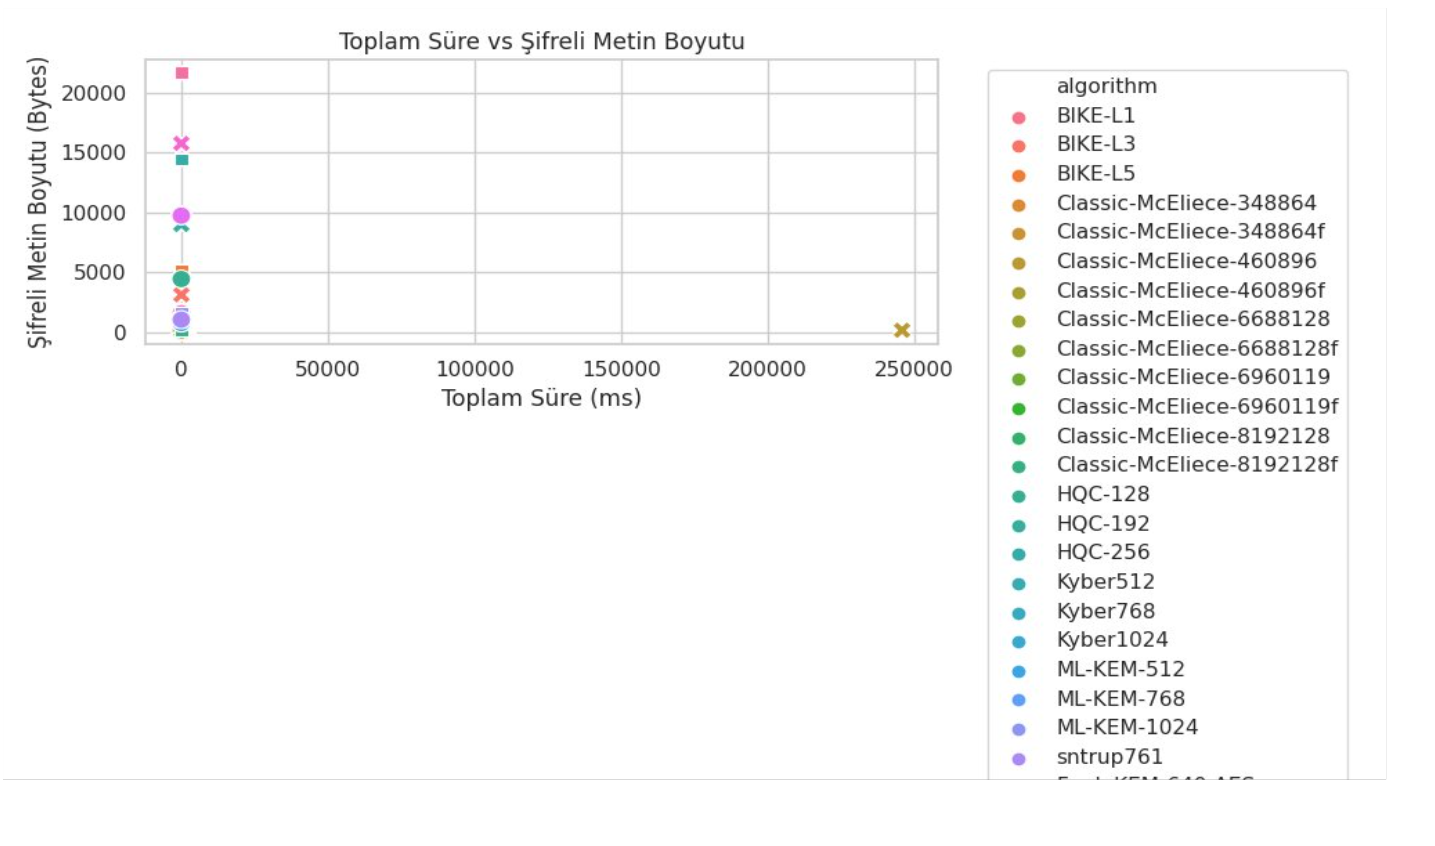
\includegraphics[width=\linewidth]{kem_performance.png}
\caption{Post-kuantum KEM benchmark verisinde toplam süre ile ciphertext boyutu arasındaki ilişki}
\label{fig:kem}
\end{figure}

\begin{table}[htbp]
\centering
\caption{Güvenlik seviyesi 1 için en hızlı 8 algoritma (ortalama)}
\label{tab:toplvl1}
\begin{tabular}{lrr}
\toprule
Algorithm & Mean Total Time (ms) & Mean Ciphertext (B) \\
\midrule
Kyber512 & 0.034 & 768 \\
ML-KEM-512 & 0.037 & 768 \\
FrodoKEM-640-AES & 0.879 & 9720 \\
sntrup761 & 1.925 & 1039 \\
HQC-128 & 2.747 & 4433 \\
FrodoKEM-640-SHAKE & 3.934 & 9720 \\
BIKE-L1 & 11.352 & 1573 \\
Classic-McEliece-348864f & 47.477 & 96 \\
\bottomrule
\end{tabular}
\end{table}

\subsection{Bulguların Yorumu}
Veri, ML-KEM/Kyber ailesinin düşük toplam süre (ms) ve makul ciphertext boyutu ile öne çıktığını göstermektedir.
Öte yandan bazı Classic McEliece varyantlarında ciphertext boyutu ve/veya toplam süre maliyeti belirgin şekilde artmaktadır.
Bu gözlem, sistem tasarımında (ör. TLS anahtar anlaşması) \emph{bant genişliği} ve \emph{hesaplama} bütçesinin güvenlik seviyesi ile birlikte değerlendirilmesi gerektiğini ortaya koyar.
Dolayısıyla tek bir ``en iyi'' algoritma yoktur; kullanım senaryosu (mobil/IoT, veri merkezi, uzun süreli arşivleme vb.) seçim üzerinde belirleyicidir.

\section{MP5: Sonuç ve Öneriler}
Kuantum bilgisayarlar, açık anahtarlı kriptografi için yapısal bir kırılma yaratmaktadır.
Bu nedenle kurumlar aşağıdaki adımları planlamalıdır:
(i) kripto envanteri çıkarımı ve kripto çevikliği,
(ii) NIST standardı PQC algoritmalarına (özellikle KEM) geçiş yol haritası,
(iii) uzun ömürlü veriler için hibrit protokoller ve anahtar uzunluğu güncellemeleri,
(iv) ``harvest-now, decrypt-later'' riskine karşı veri sınıflandırması ve yeniden şifreleme planları.
Akademik tarafta ise; gerçek donanım/implementasyon ölçümleri, yan kanal dayanımı ve protokol düzeyi etkiler (TLS, VPN, e-imza altyapıları) daha ayrıntılı incelenmelidir.

\begin{thebibliography}{10}

\bibitem{shor1994}
P. W. Shor, ``Algorithms for quantum computation: discrete logarithms and factoring,'' \emph{Proceedings 35th Annual Symposium on Foundations of Computer Science}, 1994.

\bibitem{grover1996}
L. K. Grover, ``A fast quantum mechanical algorithm for database search,'' \emph{Proceedings of the 28th Annual ACM Symposium on Theory of Computing}, 1996.

\bibitem{preskill2018}
J. Preskill, ``Quantum computing in the NISQ era and beyond,'' \emph{Quantum}, vol. 2, p. 79, 2018.

\bibitem{nistpqc}
National Institute of Standards and Technology (NIST), ``Post-Quantum Cryptography Standardization,'' project reports and documentation, 2016--2025.

\bibitem{gisin2002}
N. Gisin, G. Ribordy, W. Tittel, and H. Zbinden, ``Quantum cryptography,'' \emph{Reviews of Modern Physics}, vol. 74, no. 1, pp. 145--195, 2002.

\bibitem{kagglebench}
T. Qayyum, ``PQC Algorithms Benchmark Data (KEM performance benchmarks),'' Kaggle dataset / benchmark collection, 2025.

\end{thebibliography}

\end{document}
